% !TEX root = main.tex
\section{核心星云指数}

核心星云指数用于衡量{\textbf{一段时间内}}用户对整个经济体的贡献。
精确地计算这一指标是十分困难的,因此,我们使用了近似算法。
在该近似算法中,我们考虑了两个重要的因素,即账户持有的币龄和账户在交易网络中的位置信息。在稍后的评测中,我们将证明这种近似算法的有效性。


我们使用一段时间内链上的交易记录作为核心星云指数的数据来源。
对于一段时间$[t_0\ −\ T,\ t_0]$内的交易记录,可以描述为集合
\begin{align}
\Theta(t_0) = \{(s, t, w, \tau)\ |\ t_0 - T \le \tau \le t_0\ \land \ w > 0 \land s \neq t \}
\end{align}
\noindent 基于$\Theta(t_0)$,我们可以构造有向加权图,其中节点为账户地址,从节点$s$到节点$d$的有向边是一次交易,
边的权值为$w$,边的时间为$\tau$。


对于账户$a \in \mathcal{A}$,其核心星云指数$\mathcal{C}(a)$的计算基于$\Theta(t_0)$,即
\begin{align}
\mathcal{C}(a) = \Omega(\beta(a)) \times{} \Psi(\gamma(a))
\label{eq:rank}
\end{align}
\noindent 其中$\beta(a)$为一段时间内账户$a$持有资产的中值;$\gamma(a)$为账户$a$在一段时间内的出入度指标。

%{我们分别考虑式~\ref{eq:rank}中的三个问题,资产中值$\beta(a)$的计算,出入度指标$\gamma(a)$的计算,以及计算函数$\Omega$及$\Psi$的选择。}

%{\color{gray}注意,我们并未使用技术白皮书中的计算方法。说说原因,}

\whitepaper{相比星云技术白皮书~\cite{Nabulas}中对于星云指数的计算方法,我们做了如下改动:\\
1.在构造交易图时取消了采取最高$K$个交易额作为权值;\\
2.取消了LeaderRank中通过计算背景节点有向边权重来获取重要性评分的方式。\\
首先,我们在计算出入度指标$\beta$时采用了去环处理,因此已经可以抵抗环形转账攻击,并同时保留边的强度信息。对于存在同构图的拓扑结构,PageRank等对称函数(包括LeaderRank)被证明无法有效抵抗女巫攻击~\cite{cheng2005sybilproof}。因此在本黄皮书中我们没有采用类拓扑排名策略。在~\refsec{sec:function}中我们构造的非对称计算函数~\ref{eq:rank-param}将可以有效降低伪造低收入节点的收益。}

下面,我们将分别考虑~\ref{eq:rank}中的三个问题:资产中值$\beta(a)$的计算、出入度指标$\gamma(a)$的计算,以及函数$\Omega$及$\Psi$的选择。

\subsection{资产中值$\beta(a)$}
对于时间段$[t_0\ −\ T,\ t_0]$,区块链系统中存在$n$个区块,记为
\[
B_0, B_1, \dots, B_n
\]
\noindent 其中$B_{i}$ 为$B_{i+1}$的父块。对于账户$a \in \mathcal{A}$,其在每个区块结束后,
其相应的账户余额为
\[
d^a_0, d^a_1, \dots, d^a_n
\]
上述序列按从小到大排序后可以得到
\[
d^a_{(0)}, d^a_{(1)}, \dots, d^a_{(n)}
\]
其中$d^a_{(i)} < d^a_{(i+1)}, 0\le i \le {n-1}$,由此,可以得到
\begin{align}
\beta(a) = \left\{ \begin{array}{rcl}
{d^a_{(k)}} & \mbox{for} & n=2\times{}k, k=1, 2, 3, \ldots \\
{(d^a_{(k)} + d^a_{(k+1)})/2} & \mbox{for} & n=2\times{}k + 1, k=1, 2, 3, \ldots
\end{array}\right.
\end{align}
资产中值一定程度上代表了“币龄”,即账户中需要至少持有该资产一半以上的时间。

\subsection{出入度指标$\gamma(a)$}
考虑到恶意操控者会利用“环形转账”行为提升自己的出入度指标,因为对于出入度指标的计算首先需要对交易图进行“去交易环”处理。交易环(forwarding loop)是指一组按时间顺序进行的交易行程的环路。
一个交易环在节点$v$开始并结束,是交易图中边的集合,记为$H(v)$,即,
\[
H(v) = \{(v, v_1, w_1, \tau_1), (v_1, v_2, w_2, \tau_2), \dots, (v_i, v_{i+1}, w_{i}, \tau_i), \dots, (v_n, v, w_{n+1}, \tau_{n+1})\}
\]
\noindent 其中,$\forall 1\le i \le n : \tau_i \le \tau_{i+1} $。
\noindent 如~\ref{fig:loop}所示,包含了一个交易环,注意,其中$(v_1, v_2, 100, 5)$并不包含在交易环中。

\begin{figure}
\centering
  \begin{tikzpicture}
\pgfmathsetmacro{\XTD}{3.8}
\pgfmathsetmacro{\XMD}{1.2}
\pgfmathsetmacro{\YTD}{3.8}


\tikzset{
  node/.style={draw, circle, on grid, align=center, minimum height=2ex},
  thread/.style={draw, rectangle, on grid, align=center,color=gray!30,
  fill=gray!30,
  rounded corners,
  minimum height=3ex,fit=#1},
}

\node[node] (v) at (0, 0) {$v$};
\node[node] (v1) at (0, \YTD) {$v_1$};
\node[node] (v2) at (\XTD, \YTD) {$v_2$};
\node[node] (v3) at (\XTD, 0) {$v_3$};

\draw[->,>=stealth'] (v) to [out=135, in=225] node[left, midway] {$w=100$,$\tau=1$} (v1);
\draw[->,>=stealth'] (v1) to [out=45, in=135] node[above, midway] {$w=10$,$\tau=2$} (v2);
\draw[->,>=stealth'] (v1) to [out=315, in=225] node[below, midway] {$w=100$,$\tau=5$} (v2);
\draw[->,>=stealth'] (v2) to [out=315, in=45] node[right, midway] {$w=10$,$\tau=3$} (v3);
\draw[->,>=stealth'] (v3) to [out=225, in=315] node[below, midway] {$w=10$,$\tau=4$} (v);

\node at (2.5*\XTD, 0.5*\YTD) {
$\begin{aligned}
     H(v) = \{&(v, v1, 100, 1),\\
     &(v1, v2, 10, 2), \\
     &(v2, v3, 10, 3), \\
     &(v3, v, 10, 4) \}
  \end{aligned}$};
\end{tikzpicture}

\caption{loop\label{fig:loop}}
\end{figure}

\begin{figure}
\centering
\begin{tikzpicture}
\pgfmathsetmacro{\XTD}{3.8}
\pgfmathsetmacro{\XMD}{1.2}
\pgfmathsetmacro{\YTD}{3.8}


\tikzset{
  node/.style={draw, circle, on grid, align=center, minimum height=2ex},
  thread/.style={draw, rectangle, on grid, align=center,color=gray!30,
  fill=gray!30,
  rounded corners,
  minimum height=3ex,fit=#1},
}

\node[node] (v) at (0, 0) {$v$};
\node[node] (v1) at (0, \YTD) {$v_1$};
\node[node] (v2) at (\XTD, \YTD) {$v_2$};
\node[node] (v3) at (\XTD, 0) {$v_3$};
\draw[->,>=stealth'] (v) to [out=135, in=225] node[left, midway] {$w=90$,$\tau=1$} (v1);
\draw[->,>=stealth'] (v1) to [out=315, in=225] node[below, midway] {$w=100$,$\tau=5$} (v2);

\end{tikzpicture}
\caption{\reffig{fig:loop}去掉交易环后的交易图 \label{fig:no-loop}}
\end{figure}


在找到交易环后,需要进行去交易环处理。假设系统中存在$n$个交易环,按照交易环在交易图中出现的顺序记为
\[
H^1(v_1), H^2(v_2), \dots, H^n(v_n)\]
\noindent 其中,$H^i(v_i)$中交易金额最小的交易为 $(s^i_m, t^i_m, w^i_m, \tau^i_m)$,即
\[
\forall (s^i, t^i, w^i, \tau^i) \in \mathcal{T} : w^i \ge w^i_m
\]
\noindent 然后,需要依次将$H^i(v_i)$中所有的交易减去相应的最小交易量$w^i_m$,
如果新的交易量为0,则移除该交易,即
\[
\mathcal{E}((s, t, w, \tau), w_m) = \left\{ \begin{array}{rcl}
(s, t, w-w_m, \tau) & \mbox{if} & w \ne w_m \\
\phi & \mbox{if} & w = w_m
\end{array}\right.
\]
\begin{align}
\Theta^{\prime}(t_0)=\Theta(t_0)-H^i(v) \cup \{\mathcal{E}(t), t\in H^i(v_i)\} \quad i = 1, 2,\dots, n
\end{align}
\noindent 如~\reffig{fig:no-loop}所示,为~\reffig{fig:loop}去掉交易环之后的交易图。


%在去除所有的交易环后,对交易图中的每个节点,我们仅保留交易量最高的$k$个出边及入边,由此得到新的交易图$\Theta^{\prime\prime}(t_0)$。

记节点$v$的转入金额为$p(v)$,则
\begin{align}
p(v) = \sum_{(s_i, v, w_i, \tau_i) \in \Theta^{\prime}(t_0)}{w_i}
\end{align}
\noindent 同理,节点$v$的转出金额有
\begin{align}
q(v) = \sum_{(v, t_i, w_i, \tau_i) \in \Theta^{\prime}(t_0)}{w_i}
\end{align}
\noindent 由此,
对于节点$v$,其出入度指标$\gamma(v)$为

\begin{align}
\mathcal{G}(v) = (p(v) + q(v)) \cdot e^{-2\sin^2{(\frac{\pi}{4} - \arctan\frac{q(v)}{p(v)})}}
\end{align}
\noindent 该函数图形如~\reffig{fig-surf}所示。
\begin{figure}
  \centering
  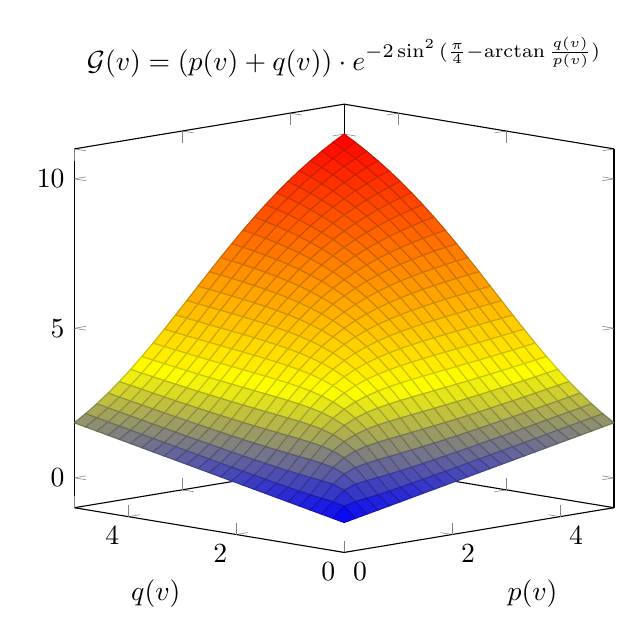
\begin{tikzpicture}[
    declare function={tf(\x)=(pi/4-rad(atan(\x)));},
    declare function={func(\x,\y)=sin(tf(\y/\x)*180/pi);}
]
\begin{axis}[
    view={315}{10},
    title={$
\mathcal{G}(v) = (p(v) + q(v)) \cdot e^{-2\sin^2{(\frac{\pi}{4} -
\arctan\frac{q(v)}{p(v)})}}$},
    xlabel=$p(v)$,
    ylabel=$q(v)$,
]

\addplot3 [
        surf,
        domain=0:5,
        domain y=0:5,
    ] {(x+y)*exp((-2)*(func(x,y))^2)};
\end{axis}
\end{tikzpicture}

\caption{出入度计算函数曲线 \label{fig-surf}}
\end{figure}

\begin{align}
\gamma(v) = (\frac{\theta\cdot \mathcal{G}(v)}{\mathcal{G}(v) + \mu})^{\lambda}
\end{align}
\noindent 其中$\theta, \mu, \lambda$为待定的参数。


\subsection{Wilbur函数 \label{sec:function}}
考虑到不同的使用场景及不同的性质,星云指数的计算是十分复杂的,然而,我们可以总结出一般意义上的星云指数计算函数的特征。

在此我们将星云指数的计算函数命名为Wilbur Function\footnote{女巫攻击(Sybil Attack)命名的来源于上世纪七十年代的美国系列电影《Sybil》,剧中患有人格分裂症的小女孩名叫Sybil,而治疗她的心理医生则名叫Dr. Cornelia Wilbur。},记为\(f(x)\),其中\(x\)
为星云指数需要参考的因素,可以为持有的余额、币龄或账户的出入度。$f(x)$需要满足两个性质:

\begin{property}
\label{prop:one}
对于任意大于$0$的两个输入变量$a$,$b$,其计算函数之和小于其和的计算函数。
%对于任意输入$x$,将其拆分后的计算函数之和小于原计算函数。
\end{property}

\begin{align}
f(a+b)>f(a)+f(b) \quad a>0,b>0
\end{align}

\begin{property}
\label{prop:two}
当任意大于$0$的两个输入变量趋近于无穷大时,其计算函数之和趋近于其和的计算函数。
\end{property}

\begin{align}
\lim\limits_{a \to \infty, b\to \infty} f(a+b) = f(a) + f(b)\quad a>0, b>0
\end{align}

\noindent 上述特性保证了在给定交易行为的情况下,用户通过控制多个账户实现该交易行为的收益小于通过单一账户实现交易的收益,同时当用户资产足够大时,其拆分账户交易的损失可以忽略不计。

\noindent 满足上述两个性质的函数有很多,在此,我们仅给出一个满足上述性质的函数,该函数的图形如~\reffig{fig-nr}所示。
\begin{align}
f(x) = x/(1 + e^{a + b\cdot x}) \quad a>1,b<0
\end{align}
\noindent {证明:详细见附录~\ref{sec:appendix_proof}}

\begin{figure}
\centering
\begin{tikzpicture}[
    declare function={func(\x,\mu) = (\x / (1 + exp(\mu-\x)));},
    declare function={linefunc(\x) = \x;}
]
\begin{axis}[
    axis lines=left,
    enlargelimits=upper,
ticks=none,axis x line=bottom,axis y line=left,xlabel={Nebulas Rank Factor},
  ylabel={星云指数},
      legend pos=north west,
legend style={fill=none}
]
\addplot [dashed, domain=0:10, blue] {linefunc(x)};
\addplot [smooth, domain=0:10, red] {func(x,3)};
\addlegendentry{$f(x)=x$}
\addlegendentry{$f(x)=x/(1 + e^{a + b\cdot x})$}
\end{axis}
\end{tikzpicture}
\caption{星云指数计算函数曲线 \label{fig-nr}}
\end{figure}


\vspace{2em}
综上,式~\ref{eq:rank}可以进一步写为

\begin{align}
\label{eq:rank-param}
\mathcal{C}(v) =  \frac{\beta(v)}{1+e^{a + b \cdot \beta(v)}} \cdot \frac{\gamma(v)}{1+e^{c + d \cdot \gamma(v)}}
\end{align}
\noindent 其中,$a, b, c, d$为待定的参数。

为了验证该函数的有效性,我们根据以太坊中的数据,计算了以太坊中地址的星云指数,并根据其市值变化计算了两者的相关性。测试数据包括了以太坊从2017年5月1日起至2017年6月30日(3629091区块至3955158区块)的所有交易记录,以及ETH日均价格(对美元)和日均总交易量~\cite{coinmarketcap}。


~\reffig{fig-eth-simu}表示了以太坊的市值与星云指数随时间变化趋势,如图所示,其中黑色标记实线为通过ETH日均交易量以及ETH日均价格计算得出的以太坊市值(对美元),而红色实线则是根据公式~\ref{eq:rank-param}计算所有以太坊用户的星云指数之和。

可以看出,星云指数能够有效反映以太坊市值变化,二者的相关系数(Correlation coefficient)为0.84427,$p$值(p-value)为$4.48\times{}10^{-17}<0.001$。说明函数~\ref{eq:rank}能够有效表示用户对整个经济体的贡献,即体现出星云指数的真实性。


\begin{figure}
\centering
\begin{tikzpicture}
  \begin{axis}[
  axis y line*=left,
  axis x line=none,
%ticks=none,
ylabel={以太坊市值(美元)},
%xtick={0,10,20,30,40,50,60},
%xlabel={时间(天)}
legend style={fill=none}
    ]
\addplot[smooth, mark=., color=red] table [x=day, y=nr, col sep=comma]
    {../common/eth_simu.csv};
\label{plot_one}

\end{axis}
  \begin{axis}[
%ticks=none,
legend pos=north west,
%ylabel={星云指数},
xlabel={时间(天)},
xtick={0,10,20,30,40,50,60},
ytick={1,2},
axis y line*=right,
legend style={fill=none}
    ]
    \addlegendimage{/pgfplots/refstyle=plot_one}\addlegendentry{星云指数}

    \addplot[smooth, mark=x] table [x=day, y=cap, col sep=comma]
    {../common/eth_simu.csv};
    \label{plot_two}
      \addlegendentry{以太坊市值}
\end{axis}

\end{tikzpicture}
\caption{以太坊之上的星云指数及以太坊市值}
\label{fig-eth-simu}
\end{figure}
